%%%%%%%%%%%%%%%%%%%%%%%%%%%%%%%%%%%%%%%%%%%%%%%%%%%%%%%%%%%%%%%%%%%%%%%%
%%
%% template.tex
%% Change Log
%% 2010-04-19 Yasuhiro Sugimoto <yas@mech.eng.osaka-u.ac.jp>
%% * 大須賀・石川研研究会資料用に修正
%%
%% 2018-1-1 Keisuke Naniwa <naniwa@es.hokudai.ac.jp>
%% * 大須賀・杉本研研究会資料用に修正
%%   osukaLab2018.styを使用することを前提にした記述とパッケージに変更
%%  いくつかのべからず集を記載してあるので,熟読の上資料作成のこと(ここすら読んでないなら知らん)
%%
%% 2020-10-23 Keisuke Naniwa <naniwa@es.hokudai.ac.jp>
%% * いまだ散見される\bfなどの記述がなぜだめなのかの例を追加
%%   
%%  
%%%%%%%%%%%%%%%%%%%%%%%%%%%%%%%%%%%%%%%%%%%%%%%%%%%%%%%%%%%%%%%%%%%%%%%%
\RequirePackage{plautopatch}%新おまじない
\RequirePackage[l2tabu, orthodox]{nag}%おまじない

\documentclass[platex,dvipdfmx]{jlreq}%ドキュメントクラスオプションの時点で,メソッドを明記しておく
\usepackage{osukalab2020}%使用前にstyファイル内を一度目を通しておくこと
\usepackage{epic,eepic}
\usepackage{graphicx}%冒頭でdvipdfmxを指定しているためここでの記述は不要
\usepackage{amsmath}	% required for `\align' (yatex added)もし必要なパッケージがインクルードされてない場合,こんな感じでやてふが自動で入れてくれます(ただし^C^Bでやった場合だけ.みんな^C^B使ってるよね・・・?)
\usepackage[all, warning]{onlyamsmath}
%\usepackage{epsfig} % このパッケージは使わずに画像の形式はPDFを使いましょう
%写真はjpg,スクショはpng,グラフやイラストはpdfで
%matlabでのグラフ出力については別で
\usepackage{siunitx} %単位や数値が綺麗に入ります
%\usepackage{times} % これもう古いのでtxfonts使おね
\usepackage{txfonts} %綺麗なtimesフォント系への切り替え
\usepackage{amssymb}
\numberwithin{equation}{section}%式がたくさん出る人はこちらをどうぞ,3章の5式目とかがeq.(3.5)とかになります


\usepackage[dvipdfmx]{hyperref}%ここら辺は本来いりませんハイパーリンク用です
\usepackage{pxjahyper}%ここら辺は本来いりませんハイパーリンク用です
\hypersetup{% hyperrefオプションリスト
setpagesize=false,
 bookmarksnumbered=true,%
 bookmarksopen=true,%
 colorlinks=true,%
 linkcolor=blue,
 citecolor=blue,
}


 
\pagestyle{empty}

\headding{大須賀・杉本研 研究会資料}
% 和文題名
\title{大須賀・杉本研 研究会資料用テンプレート}  
% 英文題名 英文題名とか,英文著者名入れたい時はosukalab2018.styの中身をいじってちょ
%\etitle{p\LaTeX-Style file for Osuka-Sugimoto Lab. Meeting}
% 著者の和文名
\author{
     浪花 啓右
     }
% 著者の英文名
%\engauthor{
%     Keisuke NANIWA
%}
% 英文の概要
\abstract{Please write your English abstract here.
}
% キーワード
\keywords{研究会資料,大須賀・杉本研,大阪大学}
%

\begin{document}
\maketitle
\thispagestyle{empty}
%
\section{はじめに}
以下に色々な例示をします.
ソースファイルと出力の関係をしっかり理解しましょう.
一部スタートダッシュ課題の解答に近いものや,解答そのものがあるので,スタートダッシュプログラムを終えてから参照する方が良いかもしれません.

\section{いろんな基本}

\subsection{文章での基本}
分野や流派によって異なりますが,基本的に句読点はカンマとピリオドを使用しましょう.
日本語の文中では,カンマとピリオドは全角,数式や英文の中では半角で記入しましょう.
また,一部漢字をなるべく使わないなどのマナーもあります.(ex.殆ど→ほとんど,最も→もっとも,など)漢字使うとかっこいいかもしれませんが,ぶっちゃけ読みづらいです(逆もまたしかりですが,あまりにもひらがなばかりだと読みにくい場合もありますよね).大切なのは指定のルールに従うことと,ルールに記載がなければあなたの采配で,資料や論文内で統一することです.
漢字かひらがなか迷ったら\href{http://www.yamanouchi-yri.com/yrihp/techwrt-2-4s/t-2-4s03a.htm}{こちらのサイト}などを参照するのも良いでしょう.


また,改行ですが\\
この方法は使わずに

このように空行を入れることで改行するようにしましょう.なぜかは出力を見ればわかるはずです.スラッシュによる改行はtabler環境内だけなどにしましょう.

また,たまに太字やイタリックを使いたくなることはあると思いますが,\textbf{こちらのやり方や,}\textit{Such a method}を使いましょう.
イタリックにしつつ太字などは\textbf{\textit{Samplle text}}とすればうまくいきます.
あなたがエディタにVSCodeを使っていて,tex環境がちゃんと整えられていれば,この文章をタイプセットしたときに,前者の書き方は警告がでるはずです.

\begin{figure}[tb]
 \centering %center環境はズレやすいから使わないこと,このようにcentering使いましょう
  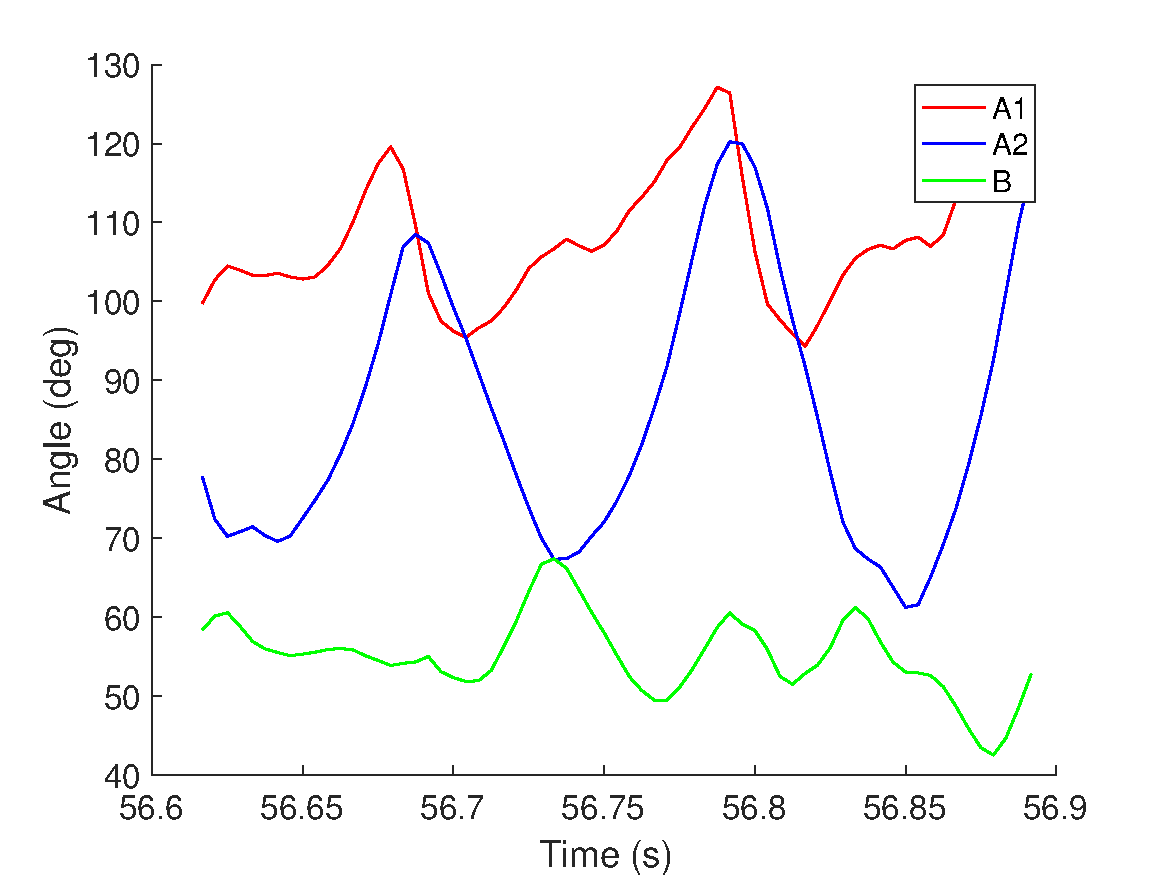
\includegraphics[width=\columnwidth]{./figure/testfig.pdf}
  \caption{参照する図にもよりますが,ここにキーとなる図があると見栄えがいいと思っています}
  \label{fig:test}
\end{figure}

\subsection{数式での基本}

数式はカギカッコもしくはalign環境で書きましょう.短く$5.0$~Vとか書きたければこんな感じで.ちなみに具体的な数字の場合は単位に括弧はつけずに,$x$~(m)とか文字の場合は括弧をつけるのがスタンダードだと思っています.単位の前には改行されない半角スペースを入れるのも忘れずに.\si{kg.m.s^{-1}}とかの単位も,\num{3.14159265e34}とか\num{.3e45}の数字もsiunitパッケージ入れてると綺麗にかけるよね.数字のリストもサポートしてくれているので\numlist{ 1.0; 2.0; 3.0; 4.0; 5.0}とか,\SIlist{ 1.0; 2.0; 3.0; 4.0; 5.0}{\volt}なんてこともできるね!でもこれ英語での場合だね.あまり気にしなくてもいいかもね.

数式は式番号いらないなら
\[
 y=\sin{A}
\] 
式番号がいるなら
\begin{align}
 y=\sin{A}
 \label{eq:test}
\end{align}
どちらの環境内でも最新のやてふなら数学記号のショートカット(セミコロンキー)やギリシャ文字のショートカット(コロンキー)に反応してくれるので安心です.
式を参照する場合は\refeq{test}とするとOK.

数式を使う人は\href{http://www.math.tohoku.ac.jp/~kuroki/LaTeX/howtolatex.html}{このサイト}も参照しましょう.


\subsection{図の基本}

スーパー何度も書いたり言ったりしてるのでさすがに大丈夫だと思いますが,
\begin{itemize}
 \item グラフや図,線描のイラストはベクタ画像であるpdf形式で
 \item 写真などはラスタ画像であるjpgで
 \item スクリーンショットはD2D(dot to dot)の画像データになるのでpngで
\end{itemize}
載せましょう.これら全ては最終出力となる書類のpdfに直接埋め込むことができるので,タイプセットも早くて楽です.

図の引用の例Fig.~\ref{fig:test}これは間違いではないけど・・・
図の引用の例\reffig{test}.%せっかくreffigあるので活用しましょう.これ使う場合はチルダ内臓されているのでチルダの入れ忘れもなくて安心

流派にもよるとは思いますが,figure環境の配置オプションはtb!ぐらいがいいと思います.
widthなども,直接値を指定する(width=3.4cmとか)はできる限りやめましょう.だいたい\verb#width=\columnwidth#でぴったり入るはずです.それがダメな場合はだいたい元画像がよくないです.元画像を修正しましょう.

\if0%$$$$$$$$$$$$$$$$$$$$$$$$$$$$$$$$$$$$$$$$$$$$$$$$$$$$$$ここからコメントアウト
%\if0と\fiで囲まれた範囲は無視されます.たくさんコメントアウトするのが大変な時に使えますが,乱用は混乱を招くので注意
\begin{figure}[tb]
 \centering %center環境はズレやすいから使わないこと,このようにcentering使いましょう
  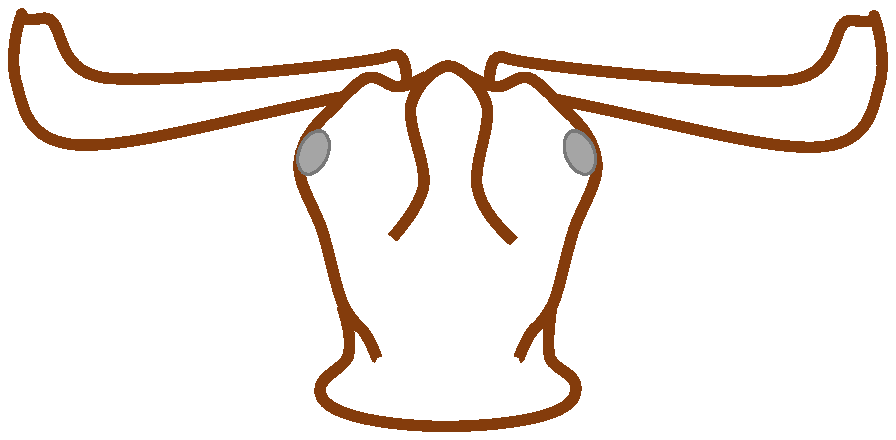
\includegraphics[width=\columnwidth]{./figure/testfig2.pdf}
  \caption{Test 2}
  \label{fig:test2}
\end{figure}
\fi%%%%%%%%%%%%%%%%%%%%%%%%%%%%%%%%%%%%%%%%%ここまでコメントアウト

複数の画像を一つのfigure環境に入れたい場合は,subfigure環境やsubfig環境は古いようです.subcaption環境を使いましょう\reffig{animals}.
こんな感じで参照も可能\reffig{frog}.

\begin{figure}[tb]
  \begin{minipage}[b]{.5\columnwidth}
   \centering
   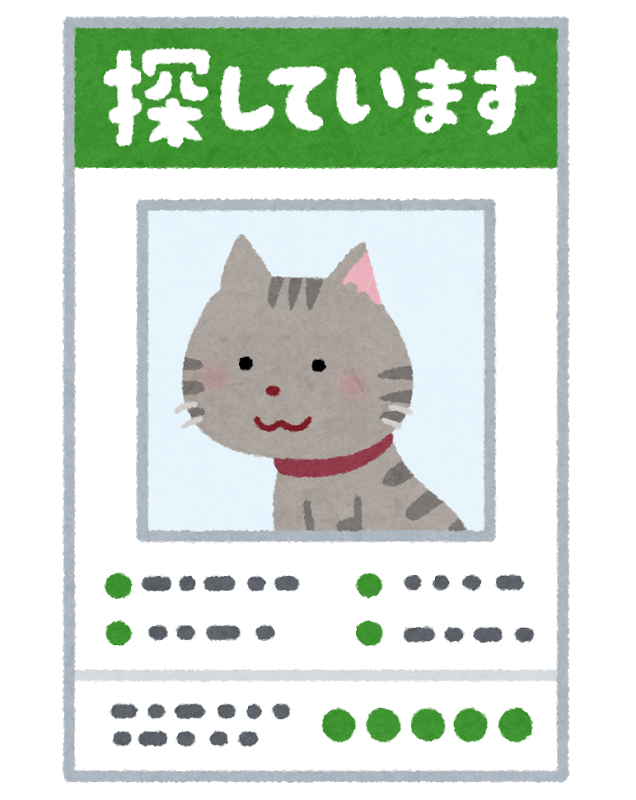
\includegraphics[width=\columnwidth]{./figure/cat.png}
   \subcaption{Tiger}
   \label{fig:frog}
 \end{minipage}%
 \begin{minipage}[b]{.5\columnwidth}
  \centering
  
\includegraphics[width=\columnwidth]{./figure/elephant.png}
  \subcaption{Bear}
  \label{fig:gorilla}
 \end{minipage}
 \caption{犬と羊}\label{fig:animals}
\end{figure}

\subsection{表の基本}

\if0%$$$$$$$$$$$$$$$$$$$$$$$$$$$$$$$$$$$$$$$$$$$$$$$$$$$$$$ここからコメントアウト
%\if0と\fiで囲まれた範囲は無視されます.たくさんコメントアウトするのが大変な時に使えますが,乱用は混乱を招くので注意
\begin{table*}[tb]
  \caption{Sample table}
   \label{table:test}
   \centering
   \begin{tabular}{cccccr}\hline
    Type & Name & Voltage & Unit & This is sample & by keisuke naniwa\\ \hline \hline
   Exp. A & 46\%& 33\%& 21\%& --& --\\ 
   Exp. B & 64\%& 9\%& 27\%& 60\%& 13\%\\ \hline    
   \end{tabular}
\end{table*}
\fi%%%%%%%%%%%%%%%%%%%%%%%%%%%%%%%%%%%%%%%%%ここまでコメントアウト

\begin{table}[tb]
  \caption{Sample table 2}
   \label{table:test2}
   \centering
   \begin{tabular}{ccc}\hline
    Type & Name & Voltage \\ \hline \hline
   Exp. A & 46\%& 33\% \\ 
   Exp. B & 64\%& 9\% \\ \hline    
   \end{tabular}
\end{table}

表はいろんな流儀がありますが,私の最近の流儀は
\begin{itemize}
 \item 罫線は横線だけかく,横線もなるべく少なくする
 \item 2段組だとだいたい半分に収まらないのでブチ抜きでかく
 \item 単位は値と合わせてかく(単位の列は作らない)
\end{itemize}
です.

シンプルなほうが綺麗でみやすいです.間違えてもパワポやエクセルで作った表の画像を貼るとかはやめましょうね.

あ,あと
参考文献は特に気にすることないと思います.
参考文献の例~\cite{mike,bibtest}.

直接記入じゃなくて,bibファイル使いましょうね.セットに一緒に入れてあるしエラーはほとんど出ないはず・・・・.

\section{いろんなパターン例}\label{sec:基本}
\subsection{節はこんな感じ}\label{sec:基本2}
\subsubsection{もういっちょ}

セクションの参照\ref{sec:基本}章です.
セクションの参照\refsec{基本} 章です.

セクションの参照\refsec{基本2} 節です.

大きな式が入ると
\begin{align}
 & \left(\frac{xdx}{dy} -\frac{ydy}{dx}\right)^{2} \ ,\ \left[\vec{F} =m\vec{a}\right] \ ,\ \left| \frac{a}{b}\right| \ \left\Vert \frac{a}{b}\right\Vert \ \left< \frac{a}{b}\right> \left\{\sqrt{a+\sqrt{a}}\rightarrow \infty \right\} 
\end{align}%
(この数式は横幅がちょっと長いから組版したときに警告が出るね!\LaTeXe はそれでも空気を読んでくれるので大丈夫だけど,あまり警告は出さないようにしようね!)

たくさん式が入ると
\begin{align}
 \nabla \cdot \mathbf{D} & =\rho \ \mathrm{and} \ \nabla \cdot \mathbf{B} =0\ \\
 \int ^{a}_{b} f'( x) dx & = f( b) -f( a)\\
 e &= \lim\limits _{n\rightarrow \infty }\left( 1+\frac{1}{n}\right)^{n}
\end{align}

そういえば,数式の記号のルールはみんなちゃんと調べてね.
たとえばよくあるミスで
\begin{align}
  sin(\theta_i) = \bar{a_{max}}
\end{align}
とかはやらないようにね(りゆうは先輩に聞いてね!)
\begin{align}
  \sin(\theta_i) = \bar{a}_{\textrm{max}}
\end{align}
こっちの方が正しいね!



\reftab{test}はぶち抜き表の例だよ.

\begin{table*}[tb]
  \caption{Sample table}
   \label{tab:test}
   \centering
   \begin{tabular}{cccccr}\hline
    Type & Name & Voltage & Unit & This is sample & by keisuke naniwa\\ \hline \hline
   Exp. A & 46\%& 33\%& 21\%& --& --\\ 
   Exp. B & 64\%& 9\%& 27\%& 60\%& 13\%\\ \hline    
   \end{tabular}
\end{table*}

\begin{itemize}
 \item これは
 \item 箇条書きの例です
 \item 段落頭と箇条書きの文字の頭が合うようにしています
 \item[壱.] とかもできます 
\end{itemize}

\begin{enumerate}
 \item これは数字での
 \item 箇条書き
 \item ですよ
\end{enumerate}

\begin{description}
 \item[一つ!] 見出しを 
 \item[二つ!] 作りたい箇条書きは
 \item[みてるー?] こうするよ 
 \item[段落を]\mbox{}\\
	    入れたかったらこうしてね
 \item[入り身]\mbox{}\\
	    取りが受けの左手側に取りの右足を滑り込ませる動作
 \item[転換]\mbox{}\\
	    取りが取りの右足中心に時計回りに$180$度回転し,受けの姿勢を崩す動作
\end{description}



\begin{quotation}
 引用先から文章をそのまま引用するときはこの環境下で書くよ
\end{quotation}

  
\section*{謝辞とか}

\LaTeXe 環境の日本語化やらなんやらもう色々に尽力された奥村先生\cite{okumura7th},いつも私たちのことを先読みで色々用意してくださっている丸田先生,そのほかにもあげ始めたらキリがない先達者の方々には強く感謝しましょう.足を向けて寝てはいけません.立ったまま寝ましょう.

\appendix
\section{付録とか入れたいときはこうしよう}

これだけ偉そうに\LaTeXe のアレヤコレヤ書いてますが,ぶっちゃけ私も学生の頃は全然よくわかってなかったし,特に教えてくれる人もいませんでした.
最初にやてふ周りのことを教えてくれたのが杉本先生だったかな?それぐらいです.
さらには今回の資料を書くのにもかなり色々調べました.おかげで大変勉強になりました.まるで昔から知ってたように全部書いてますが,最近やたった今知ったばかりのにわか知識もたくさん入ってます.

なので,私が望むことは,これを読んでいるあなたにも,ぜひ自分で勉強して,そこからさらに新しく,最新で,みんなが楽になる美しい文章をかけるように努力してくれることです.
私の書いたテンプレートや,スタイルファイルをみて,矛盾した書き方や,重複,本来の書き方ではない書き方,サポートの切れた古いパッケージを未だに使っている,最新のパッケージではサポートされていることを手動で行なっている,そんな粗がたくさん見つかるようになってください.

たかが文章を書くだけでなんでそんな努力をせんといかんのや,wordなら書いたままプリントアウトできるで.という方もいらっしゃるでしょう.そういう方はもうそれでいいです.
ただ,私はレイアウトや組版規則のプロではないので美しいレイアウトの文章を自分では作れません.ですが\TeX を最新のプロの知識が反映されている状態で正しく使えば,自身がレイアウトのことを気にすることなく,読み手に優しい美しい文章がかけます.それって素晴らしいと思いませんか?

今はわからなくても,人の文章をよく読むようになった頃に,このことを少しでも思い出してくれると幸いです.浪花(2018/1/4)



%
% 以下に文献を書きます。
%
{\small
\bibliographystyle{osukalab}
\bibliography{myref}


\clearpage

\end{document}

